\documentclass{../../slides-style}

\slidetitle[Делегаты, события, лямбда-функции]{Событийно-ориентированное программирование}{28.03.2025}

\begin{document}

    \begin{frame}[plain]
        \titlepage
    \end{frame}

    \begin{frame}
        \frametitle{Событийно-ориентированное программирование: зачем?}
        \begin{itemize}
            \item Большая часть приложений большую часть времени чего-то ждёт
            \item Активное ожидание потребляет системные ресурсы
            \item Приложения с пользовательским интерфейсом:
            \begin{itemize}
                \item Цикл обработки событий
                \item Очередь событий
                \item Обработчики
            \end{itemize}
            \item Сетевые и распределённые приложения
            \item Приложения, работающие с оборудованием
        \end{itemize}
    \end{frame}

    \begin{frame}
        \frametitle{Реализация}
        \begin{itemize}
            \item Callback-и (hooks)
            \item Переопределение виртуальных методов библиотечного класса
            \begin{itemize}
                \item Inversion of Control --- не мы вызываем библиотеку, а она нас
            \end{itemize}
            \item Языковая поддержка --- event-ы
            \item Паттерн \enquote{Наблюдатель}
        \end{itemize}
    \end{frame}

    \begin{frame}
        \frametitle{Паттерн \enquote{Наблюдатель}}
        \begin{center}
            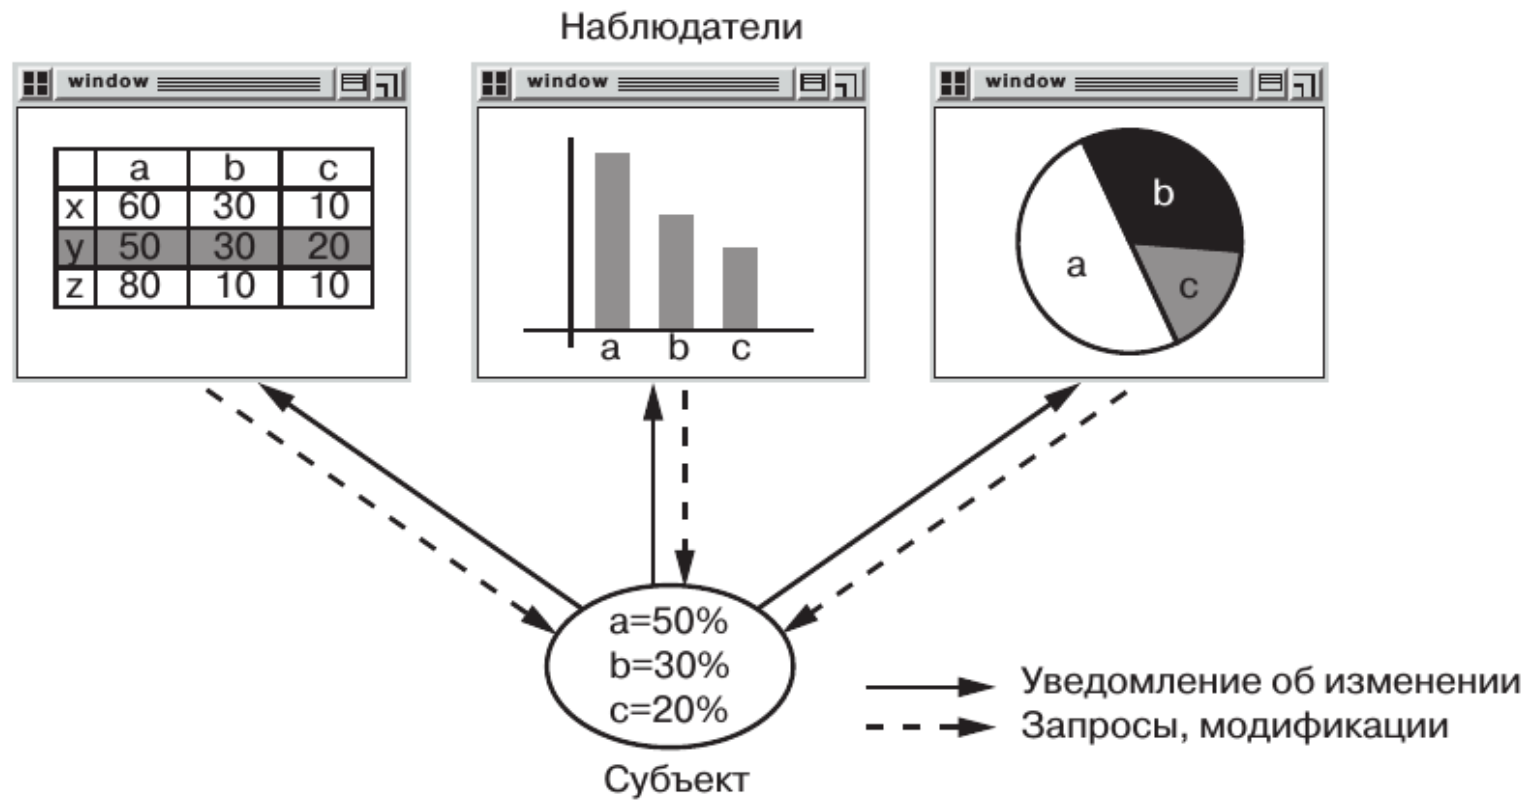
\includegraphics[width=0.9\textwidth]{observerExample.png}
        \end{center}
    \end{frame}

    \begin{frame}
        \frametitle{Наблюдатель, структура классов}
        \begin{center}
            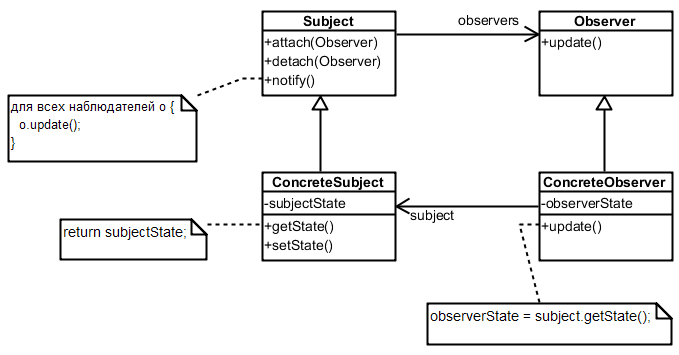
\includegraphics[width=0.8\textwidth]{observer.png}
        \end{center}
    \end{frame}

    \begin{frame}[fragile]
        \frametitle{Делегаты}
        \begin{minted}{csharp}
public delegate void Feedback(Int32 value);
        \end{minted}
        \begin{itemize}
            \item Типобезопасный callback
            \item \mintinline{csharp}|delegate| объявляет тип функции-делегата
            \begin{itemize}
                \item На самом деле, автоматически генерируемый класс
                \item Наследник System.MulticastDelegate, который в свою очередь наследник System.Delegate
                \item Методы Invoke, BeginInvoke, EndInvoke
            \end{itemize}
        \end{itemize}
    \end{frame}

    \begin{frame}[fragile]
        \frametitle{Пример использования}
        \begin{scriptsize}
            \begin{minted}{csharp}
public delegate int HashFunction(string str, int hashSize);

private static class HashFunctions {
    public static int Hash1(string str, int hashSize) {
        return str[0] % hashSize;
    }

    public static int Hash2(string str, int hashSize) {
        int result = 0;
        foreach (var ch in str)
            result += ch;
        return result % hashSize;
    }
}

static void Main(string[] args) {
    var h = new HashFunction(HashFunctions.Hash1);
    var result = h("ololo", 10);
}
            \end{minted}
        \end{scriptsize}
    \end{frame}

    \begin{frame}[fragile]
        \frametitle{Ещё пример, который будем дальше мучить}
        \framesubtitle{Цикл обработки событий}
        \begin{footnotesize}
            \begin{minted}{csharp}
public class EventLoop {
    public void Run() {
        while (true) {
            var key = Console.ReadKey();
            switch (key.Key) {
                case ConsoleKey.LeftArrow:
                    // Сделать что-то по нажатию на "влево"
                    break;
                case ConsoleKey.RightArrow:
                    // Сделать что-то по нажатию на "вправо"
                    break;
            }
        }
    }
}
            \end{minted}
        \end{footnotesize}
    \end{frame}

    \begin{frame}[fragile]
        \frametitle{Использование}
        \begin{minted}{csharp}
static void Main(string[] args)
{
    var eventLoop = new EventLoop();
    eventLoop.Run();
}
        \end{minted}
    \end{frame}

    \begin{frame}[fragile]
        \frametitle{Цикл с делегатом}
        \begin{footnotesize}
            \begin{minted}{csharp}
public delegate void ArrowHandler();

public class EventLoop {
    public void Run(ArrowHandler left, ArrowHandler right) {
        while (true) {
            var key = Console.ReadKey(true);
            switch (key.Key) {
                case ConsoleKey.LeftArrow:
                    left();
                    break;
                case ConsoleKey.RightArrow:
                    right();
                    break;
            }
        }
    }
}
            \end{minted}
        \end{footnotesize}
    \end{frame}

    \begin{frame}[fragile]
        \frametitle{Обработчики}
        \begin{minted}{csharp}
public class Game
{
    public void OnLeft()
        => Console.WriteLine("Going left");

    public void OnRight()
        => Console.WriteLine("Going right");
}
        \end{minted}
    \end{frame}

    \begin{frame}[fragile]
        \frametitle{Main}
        \begin{minted}{csharp}
static void Main(string[] args)
{
    var eventLoop = new EventLoop();
    var game = new Game();
    eventLoop.Run(
        new ArrowHandler(game.OnLeft), 
        new ArrowHandler(game.OnRight)
    );
}
        \end{minted}
    \end{frame}

    \begin{frame}[fragile]
        \frametitle{Delegate chaining}
        \begin{minted}{csharp}
public void Register(SomeDelegateType someDelegate)
    => currentDelegate = Delegate.Combine(currentDelegate, someDelegate);
        \end{minted}
        \vspace{3mm}
        Или
        \begin{minted}{csharp}
public void Register(SomeDelegateType someDelegate)
    => currentDelegate += someDelegate;
        \end{minted}
    \end{frame}

    \begin{frame}[fragile]
        \frametitle{Цикл обработки событий с регистрацией (1)}
        \begin{minted}{csharp}
public class EventLoop
{
    private ArrowHandler leftHandler;
    private ArrowHandler rightHandler;

    public void RegisterLeftHandler(ArrowHandler left)
        => leftHandler += left;

    public void RegisterRightHandler(ArrowHandler right)
        => rightHandler += right;
        \end{minted}
    \end{frame}

    \begin{frame}[fragile]
        \frametitle{Цикл обработки событий с регистрацией (2)}
        \begin{minted}{csharp}
    public void Run() {
        while (true) {
            var key = Console.ReadKey(true);
            switch (key.Key) {
                case ConsoleKey.LeftArrow:
                    if (leftHandler != null)
                        leftHandler();
                    break;
                case ConsoleKey.RightArrow:
                    if (rightHandler != null)
                        rightHandler();
                    break;
            }
        }
    }
}
        \end{minted}
    \end{frame}

    \begin{frame}[fragile]
        \frametitle{Логгер (ещё один наблюдатель)}
        \begin{minted}{csharp}
public class Logger
{
    private List<string> log = new();

    public void LeftPressed()
        => log.Add("left");

    public void RightPressed()
        => log.Add("right");
}
        \end{minted}
    \end{frame}

    \begin{frame}[fragile]
        \frametitle{Main}
        \begin{minted}{csharp}
static void Main(string[] args)
{
    var eventLoop = new EventLoop();
    var game = new Game();
    var logger = new Logger();

    eventLoop.RegisterLeftHandler(game.OnLeft);
    eventLoop.RegisterRightHandler(game.OnRight);

    eventLoop.RegisterLeftHandler(logger.LeftPressed);
    eventLoop.RegisterRightHandler(logger.RightPressed);

    eventLoop.Run();
}
        \end{minted}
    \end{frame}

    \begin{frame}[fragile]
        \frametitle{Отписывание от событий}
        \begin{minted}{csharp}
public void UnregisterLeftHandler(ArrowHandler left)
    => leftHandler = (ArrowHandler)Delegate.Remove(leftHandler , left);
        \end{minted}
        \vspace{3mm}
        или
        \begin{minted}{csharp}
public void UnregisterLeftHandler(ArrowHandler left)
    => leftHandler -= left;
        \end{minted}
    \end{frame}

    \begin{frame}[fragile]
        \frametitle{Как примерно выглядит Invoke для цепочки}
        \begin{minted}{csharp}
public int Invoke(int value) {
    int result;
    Delegate[] delegateSet = _invocationList as Delegate[];
    if (delegateSet != null) {
        foreach (Feedback d in delegateSet)
            result = d(value);
    } else {
        result = _methodPtr.Invoke(_target, value);
    }

    return result;
}
        \end{minted}
    \end{frame}

    \begin{frame}[fragile]
        \frametitle{Вызов делегатов из цепочки вручную}
        \begin{small}
            \begin{minted}{csharp}
Delegate[] arrayOfDelegates = leftHandler.GetInvocationList();
foreach (ArrowHandler handler in arrayOfDelegates) {
    try {
        handler.Invoke();
    }
    catch (InvalidOperationException e) {
        Object component = handler.Target;
        Console.WriteLine(
                "Failed to call handler from {1}{2}{0} Error: {3}{0}{0}",
                Environment.NewLine,
                ((component == null) ? "" : component.GetType() + "."),
                handler.GetMethodInfo().Name,
                e.Message);
    }
}
            \end{minted}
        \end{small}
    \end{frame}

    \begin{frame}[fragile]
        \frametitle{Шаблонные типы делегатов}
        \begin{minted}{csharp}
public delegate int HashFunction(string str, int hashSize);
        \end{minted}
        \hspace{2cm}\begin{Large}$\downarrow$\end{Large}
        \begin{minted}{csharp}
Func<string, int, int>
        \end{minted}
        \begin{itemize}
            \item \mintinline{csharp}|Func<T1, T2, ..., TResult>|
            \item \mintinline{csharp}|Action<T1, T2, ...>|
            \item Не дружат с \mintinline{csharp}|ref| и \mintinline{csharp}|out|
        \end{itemize}
    \end{frame}

    \begin{frame}[fragile]
        \frametitle{События}
        \mintinline{csharp}|eventLoop.RegisterLeftHandler(game.OnLeft);| --- много работы

        \mintinline{csharp}|eventLoop.leftHandler += game.OnLeft;| --- очень плохо

        \vspace{3mm}
        Надо (в EventLoop):
        \begin{minted}{csharp}
public event Action LeftHandler;
public event Action RightHandler;
        \end{minted}
        \vspace{3mm}
        и (в Main):
        \begin{minted}{csharp}
eventLoop.LeftHandler += game.OnLeft;
eventLoop.RightHandler += game.OnRight;

eventLoop.LeftHandler += logger.LeftPressed;
eventLoop.RightHandler += logger.RightPressed;
        \end{minted}
    \end{frame}

    \begin{frame}[fragile]
        \frametitle{Анонимные методы}
        \begin{minted}{csharp}
static void Main(string[] args) {
    var eventLoop = new EventLoop();
    var game = new Game();
    eventLoop.LeftHandler += game.OnLeft;
    eventLoop.RightHandler += game.OnRight;
    var log = new List<string>();
    eventLoop.LeftHandler += delegate {
        log.Add("left");
    };
    eventLoop.RightHandler += delegate {
        log.Add("right");
    };
    eventLoop.Run();
}
        \end{minted}
    \end{frame}

    \begin{frame}[fragile]
        \frametitle{Замыкания (1)}
        \begin{minted}{csharp}
static Func<Point, Point> CreateRemapFunction(
        Rectangle rect1, Rectangle rect2)
{
    var xScale = rect2.Width() / rect1.Width();
    var yScale = rect2.Height() / rect1.Height();
    Func<Point, Point> result = delegate(Point point) {
        var returnValue = new Point();
        returnValue.x = point.x * xScale;
        returnValue.y = point.y * yScale;
        return returnValue;
    };
    return result;
}
        \end{minted}
    \end{frame}

    \begin{frame}[fragile]
        \frametitle{Замыкания (2, пример использования)}
        \begin{small}
            \begin{minted}{csharp}
static void Main(string[] args) {
    var rect1 = new Rectangle() {
        topLeft = new Point() { x = 0, y = 0 },
        bottomRight = new Point() { x = 2, y = 2 }
    };
    var rect2 = new Rectangle() {
        topLeft = new Point() { x = 0, y = 0 },
        bottomRight = new Point() { x = 4, y = 6 }
    };

    var remap = CreateRemapFunction(rect1, rect2);
    var point = new Point() { x = 1, y = 1 };
    var transformedPoint = remap(point);
    Console.WriteLine("Transformed point: x = {0}, y = {1}", 
          transformedPoint.x, transformedPoint.y);
}
            \end{minted}
        \end{small}
    \end{frame}

    \begin{frame}[fragile]
        \frametitle{Замыкания, способ прострелить себе ногу}
        \begin{small}
            \begin{minted}{csharp}
delegate void F();

class Program
{
    static void Main(string[] args)
    {
        var delegates = new F[10];
        for (var i = 0; i < 10; ++i)
        {
            delegates[i] = delegate { Console.WriteLine(i); };
        }

        foreach (var f in delegates)
        {
            f();
        }
    }
}
            \end{minted}
        \end{small}
    \end{frame}

    \begin{frame}[fragile]
        \frametitle{Что генерит компилятор}
        \begin{scriptsize}
            \begin{minted}{csharp}
private static void Main(string[] args)
{
    F[] fArray = new F[10];
    Program.<>c__DisplayClass0_0 cDisplayClass00 = new Program.<>c__DisplayClass0_0();
    for (cDisplayClass00.i = 0; cDisplayClass00.i < 10; ++cDisplayClass00.i) {
        fArray[cDisplayClass00.i] = new F((object) cDisplayClass00, __methodptr(<Main>b__0));
    }
    foreach (F f in fArray)
        f();
}

[CompilerGenerated]
private sealed class <>c__DisplayClass0_0
{
    public int i;
    internal void <Main>b__0() {
        Console.WriteLine(this.i);
    }
}
            \end{minted}
        \end{scriptsize}
    \end{frame}

    \begin{frame}[fragile]
        \frametitle{Как бороться}
        \begin{small}
            \begin{minted}{csharp}
delegate void F();

class Program
{
    static void Main(string[] args)
    {
        var delegates = new F[10];
        for (var i = 0; i < 10; ++i)
        {
            var localI = i;
            delegates[i] = delegate { Console.WriteLine(localI); };
        }

        foreach (var f in delegates)
        {
            f();
        }
    }
}
            \end{minted}
        \end{small}
    \end{frame}

    \begin{frame}[fragile]
        \frametitle{Что получится}
        \begin{scriptsize}
            \begin{minted}{csharp}
private static void Main(string[] args)
{
    F[] fArray = new F[10];
    for (int index = 0; index < 10; ++index) {
        Program.<>c__DisplayClass0_0 cDisplayClass00 = new Program.<>c__DisplayClass0_0();
        cDisplayClass00.localI = index;
        fArray[index] = new F((object) cDisplayClass00, __methodptr(<Main>b__0));
    }
    foreach (F f in fArray)
        f();
}

[CompilerGenerated]
private sealed class <>c__DisplayClass0_0
{
    public int localI;
    internal void <Main>b__0() {
        Console.WriteLine(this.localI);
    }
}
            \end{minted}
        \end{scriptsize}
    \end{frame}

    \begin{frame}[fragile]
        \frametitle{Лямбда-выражения}
        \begin{minted}{csharp}
delegate(список параметров)
{
    тело
};
        \end{minted}
        \hspace{2cm}\begin{LARGE}$\downarrow$\end{LARGE}
        \begin{minted}{csharp}
(список параметров) => { тело };
        \end{minted}
    \end{frame}

    \begin{frame}[fragile]
        \frametitle{Примеры}
        \begin{minted}{csharp}
eventLoop.LeftHandler += () => log.Add("left");
eventLoop.RightHandler += () => log.Add("right");

Func<int, int> x2 = x => x * 2;
var n = x2(1);  // n будет 2

List<int> list = new List<int>() { 20, 1, 4, 8, 9, 44 };
List<int> evenNumbers = list.FindAll(i => (i % 2) == 0);
        \end{minted}
    \end{frame}

    \begin{frame}[fragile]
        \frametitle{Каноничное объявление события (1)}
        Наследник EventArgs, содержащий в себе параметры события
        \begin{itemize}
            \item Если параметров нет, то обработчики события всё равно должны принимать EventArgs
            \begin{itemize}
                \item Передавать при вызове имеет смысл EventArgs.Empty
            \end{itemize}
        \end{itemize}

        \vspace{3mm}
        \begin{minted}{csharp}
internal class NewMailEventArgs : EventArgs {
    private readonly string from, to, subject;
    public NewMailEventArgs(string from, string to, string subject) {
        this.from = from; this.to = to; this.subject = subject;
    }
    public string From => from;
    public string To => to;
    public string Subject => subject;
}
        \end{minted}
    \end{frame}

    \begin{frame}[fragile]
        \frametitle{Каноничное объявление события (2)}
        Само событие в наблюдаемом классе
        \begin{itemize}
            \item Инстанциация шаблона EventHandler
            \item 
                \begin{minted}{csharp}
public delegate void EventHandler<TEventArgs>(
        object sender, TEventArgs e);
                \end{minted}
        \end{itemize}

        \vspace{7mm}
        \begin{minted}{csharp}
internal class MailManager {
    public event EventHandler<NewMailEventArgs> NewMail;
    ...
}
        \end{minted}
    \end{frame}

    \begin{frame}[fragile]
        \frametitle{Каноничное объявление события (3)}
        Вспомогательный метод, кидающий событие
        \begin{itemize}
            \item Сюда идёт проверка списка подписчиков на null
            \item Вызов лучше делать потокобезопасным
        \end{itemize}
        \vspace{5mm}
        \begin{minted}{csharp}
internal class MailManager {
    ...
    protected virtual void OnNewMail(NewMailEventArgs e) {
        EventHandler<NewMailEventArgs> temp = 
                Volatile.Read(ref NewMail);
        if (temp != null) 
            temp(this, e);
    }
    ...
}
        \end{minted}
    \end{frame}

    \begin{frame}[fragile]
        \frametitle{Каноничное объявление события (4)}
        Кидание события
        \begin{itemize}
            \item Создаём наследника EventArgs
            \item Вызываем метод, отправляющий событие наблюдателям
        \end{itemize}
        \vspace{5mm}
        \begin{minted}{csharp}
internal class MailManager {
    public void SimulateNewMail(string from, string to, string subject) {
        NewMailEventArgs e = new NewMailEventArgs(from, to, subject);
        OnNewMail(e);
    }
}
        \end{minted}
    \end{frame}

    \begin{frame}[fragile]
        \frametitle{Принимающий событие}
        \begin{minted}{csharp}
internal sealed class Fax {
    public Fax(MailManager mm)
        => mm.NewMail += FaxMsg;

    private void FaxMsg(object sender, NewMailEventArgs e) {
        Console.WriteLine("Faxing mail message:");
        Console.WriteLine(" From={0}, To={1}, Subject={2}",
                e.From, e.To, e.Subject);
    }

    public void Unregister(MailManager mm)
        => mm.NewMail -= FaxMsg;
}
        \end{minted}
    \end{frame}

    \begin{frame}[fragile]
        \frametitle{Ручное управление подписчиками}
        \begin{minted}{csharp}
public event EventHandler<FooEventArgs> Foo {
    add { eventSet.Add(fooEventKey, value); }
    remove { eventSet.Remove(fooEventKey, value); }
}

protected virtual void OnFoo(FooEventArgs e) {
    eventSet.Raise(fooEventKey, this, e);
}
        \end{minted}
        \vspace{7mm}
        eventSet --- рукописный словарь с цепочками обработчиков, не поместившийся в презентацию
    \end{frame}

    \begin{frame}[fragile]
        \frametitle{Результат (1)}
        \begin{footnotesize}
            \begin{minted}{csharp}
public class EventLoop {
    public event EventHandler<EventArgs> LeftHandler = (sender, args) => { };
    public event EventHandler<EventArgs> RightHandler = (sender, args) => { };
    public void Run() {
        while (true) {
            var key = Console.ReadKey(true);
            switch (key.Key) {
                case ConsoleKey.LeftArrow:
                    LeftHandler(this, EventArgs.Empty);
                    break;
                case ConsoleKey.RightArrow:
                    RightHandler(this, EventArgs.Empty);
                    break;
            }
        }
    }
}
            \end{minted}
        \end{footnotesize}
    \end{frame}

    \begin{frame}[fragile]
        \frametitle{Результат (2)}
        \begin{footnotesize}
            \begin{minted}{csharp}
public class Game
{
    public void OnLeft(object sender, EventArgs args)
        => Console.WriteLine("Going left");

    public void OnRight(object sender, EventArgs args)
        => Console.WriteLine("Going right");
}
            \end{minted}
        \end{footnotesize}
    \end{frame}

    \begin{frame}[fragile]
        \frametitle{Результат (3)}
        \begin{footnotesize}
            \begin{minted}{csharp}
static void Main(string[] args)
{
    var eventLoop = new EventLoop();
    var game = new Game();
    eventLoop.LeftHandler += game.OnLeft;
    eventLoop.RightHandler += game.OnRight;

    var log = new List<string>();

    eventLoop.LeftHandler += (sender, eventArgs) => log.Add("left");
    eventLoop.RightHandler += (sender, eventArgs) => log.Add("right");

    eventLoop.Run();
}
            \end{minted}
        \end{footnotesize}
    \end{frame}

\end{document}
